\documentclass[10pt]{beamer}

\usepackage[]{graphicx}
\usepackage[]{color}

\usepackage{alltt}

% Beamer themer
%\usetheme{metropolis}
\usetheme{Warsaw}

\setbeamertemplate{footline}[frame number]

\usepackage{graphicx}

\DeclareGraphicsExtensions{.pdf,.jpeg,.jpg,.png}

\usepackage{subcaption}
\usepackage{amsmath}

\usepackage[authoryear]{natbib}

\usepackage{tikz}
% \usetikzlibrary{bayesnet}
\usepackage{pgfplots}
\pgfplotsset{compat=1.13}

\usepackage[framemethod=TikZ, xcolor=RGB]{mdframed}
\definecolor{mydarkblue}{rgb}{0,.06,.5}
\definecolor{mydarkred}{rgb}{.5,0,.1}
\definecolor{myroyalblue}{rgb}{0,.1,.8}
\mdfdefinestyle{MyFrame}{%
    linecolor=mydarkblue,
    outerlinewidth=0.5pt,
    roundcorner=2pt,
    innertopmargin=2pt,
    innerbottommargin=2pt,
    innerrightmargin=2pt,
    innerleftmargin=2pt,
    backgroundcolor=blue!10}

% Set a transparent background to match ggplot figures
\setbeamercolor{background canvas}{bg=}

\usepackage{xargs} % For def with default arguments
\usepackage{mathrsfs} % For mathscr

\usepackage{amssymb}
\usepackage{amsmath}
\usepackage{amsthm}
\usepackage{mathtools}

% https://tex.stackexchange.com/questions/89166/centering-in-tabularx-and-x-columns
\usepackage{tabularx}   % For horizontally filled tables
\newcolumntype{Y}{>{\centering\arraybackslash}X}
\usepackage{booktabs}    % For toprule among other things

\usepackage{refstyle}
\usepackage{varioref} % Use refstyle instead of varioref directly.

% Math definitions

% Some definitions for the text

\def\loset{MIS}
\def\loeff{MIP}
\def\loalpha{PIP}
\def\aloset{AMIS}
\def\aloeff{AMIP}
\def\aloalpha{APIP}
\def\na{\texttt{NA}}

%%%%%%%%%%%%%%%%%%%%%%%%
% Rachael's math defs

\DeclareMathOperator*{\argmax}{arg\,max}
\DeclareMathOperator*{\argmin}{arg\,min}

\DeclarePairedDelimiter\abs{\lvert}{\rvert}
\DeclarePairedDelimiter\norm{\lVert}{\rVert}

% Swap the definition of \abs* and \norm*, so that \abs
% and \norm resizes the size of the brackets, and the
% starred version does not.
\makeatletter
\let\oldabs\abs
\def\abs{\@ifstar{\oldabs}{\oldabs*}}

%\let\oldnorm\norm
\def\norm{\@ifstar{\oldnorm}{\oldnorm*}}

%%%%%%%%%%%%%%%%%%%%%%%%
% Ryan's math defs


% \norm was taken, so use \vnorm for "vector norm".
\global\long\def\info{\mathcal{I}}%

% These are all used for the finite sample bounds section.
\global\long\def\betalin{\hat\beta^{\mathrm{lin}}}%
\global\long\def\nset{\mathcal{S}}%

\global\long\def\cop{C_{op}}%
\global\long\def\cmoment{H_2}%
\global\long\def\cxxlo{\xi_1}%
\global\long\def\cxepslo{\xi_2}%
\global\long\def\cball{\mathscr{B}}%
\global\long\def\cijdiff{\Delta_{lin}}%

\global\long\def\copscaled{\tilde{C}_{op}}%

% calculus
\newcommand{\dee}{\mathrm{d}}

% Influence score and related quantities
\def\infl{\psi}
\def\inflscale{\hat{\sigma}_{\infl}}
\def\inflscalelim{\sigma_{\infl}}
\def\ind#1{\mathbb{I}\left(#1\right)}
\def\mis#1{S_{#1}}
\def\mip#1{\Psi_{#1}}
\def\amis#1{\hat{S}_{#1}}
\def\amip#1{\hat{\Psi}_{#1}}
\def\loprop#1{\alpha^*_{#1}}
\def\aloprop#1{\hat{\alpha}^*_{#1}}
\def\thetafun{\phi}
\def\thetafunlin{\thetafun^{\mathrm{lin}}}%
\def\thetalin{\thetahat^{\mathrm{lin}}}%

\def\shape{\mathcal{S}_\alpha}
\def\noise{\hat\sigma_{\phi}}
\def\plim{\overset{p}{\rightarrow}}

% Vectors
%\def\x{\vec{x}}
\def\d{d} % A general data point
\def\p{p} % The index into the parameter vector
\def\P{P} % The length of the parameter vector
\def\w{\vec{w}}
\def\wnorm{\vec{\omega}} % Used only in the \thetafun lemma

\def\zP{0_{\P}}
\def\zPN{0_{\P \times N}}
\def\thetahat{\hat{\theta}}
\def\onevec{\vec{1}}
\def\inflvec{\vec{\infl}}

% Operators
\def\sumn{\sum_{n=1}^N}
\def\meann{\frac{1}{N}\sum_{n=1}^N}
\def\var#1{\mathrm{Var}\left(#1\right)}
\def\vnorm#1{\left\Vert #1\right\Vert }%
\def\falphanorm#1#2{\left\Vert #2\right\Vert_{#1, \alpha} }%
\def\at#1#2{\left.#1\right|_{#2}}%
\def\fracat#1#2#3{\at{\frac{#1}{#2}}{#3}}%
\def\mbe{\mathbb{E}}%
\def\argmaxover#1{\underset{#1}{\mathrm{argmax}}\,}
\def\maxover#1{\underset{#1}{\mathrm{max}}\,}

% This file contains the boilerplate that knitr would put at the top of
% a knitr document if you ran knitr with \begin{document} ... \end{document}.
% By including it once in the main document, you can knit and \input{}
% Rnw files that contain only individual sections.

\usepackage[]{graphicx}
\usepackage[]{color}
%% maxwidth is the original width if it is less than linewidth
%% otherwise use linewidth (to make sure the graphics do not exceed the margin)
\makeatletter
\def\maxwidth{ %
  \ifdim\Gin@nat@width>\linewidth
    \linewidth
  \else
    \Gin@nat@width
  \fi
}
\makeatother

\definecolor{fgcolor}{rgb}{0.345, 0.345, 0.345}
\newcommand{\hlnum}[1]{\textcolor[rgb]{0.686,0.059,0.569}{#1}}%
\newcommand{\hlstr}[1]{\textcolor[rgb]{0.192,0.494,0.8}{#1}}%
\newcommand{\hlcom}[1]{\textcolor[rgb]{0.678,0.584,0.686}{\textit{#1}}}%
\newcommand{\hlopt}[1]{\textcolor[rgb]{0,0,0}{#1}}%
\newcommand{\hlstd}[1]{\textcolor[rgb]{0.345,0.345,0.345}{#1}}%
\newcommand{\hlkwa}[1]{\textcolor[rgb]{0.161,0.373,0.58}{\textbf{#1}}}%
\newcommand{\hlkwb}[1]{\textcolor[rgb]{0.69,0.353,0.396}{#1}}%
\newcommand{\hlkwc}[1]{\textcolor[rgb]{0.333,0.667,0.333}{#1}}%
\newcommand{\hlkwd}[1]{\textcolor[rgb]{0.737,0.353,0.396}{\textbf{#1}}}%
\let\hlipl\hlkwb

\usepackage{framed}
\makeatletter
\newenvironment{kframe}{%
 \def\at@end@of@kframe{}%
 \ifinner\ifhmode%
  \def\at@end@of@kframe{\end{minipage}}%
  \begin{minipage}{\columnwidth}%
 \fi\fi%
 \def\FrameCommand##1{\hskip\@totalleftmargin \hskip-\fboxsep
 \colorbox{shadecolor}{##1}\hskip-\fboxsep
     % There is no \\@totalrightmargin, so:
     \hskip-\linewidth \hskip-\@totalleftmargin \hskip\columnwidth}%
 \MakeFramed {\advance\hsize-\width
   \@totalleftmargin\z@ \linewidth\hsize
   \@setminipage}}%
 {\par\unskip\endMakeFramed%
 \at@end@of@kframe}
\makeatother

\definecolor{shadecolor}{rgb}{.97, .97, .97}
\definecolor{messagecolor}{rgb}{0, 0, 0}
\definecolor{warningcolor}{rgb}{1, 0, 1}
\definecolor{errorcolor}{rgb}{1, 0, 0}
\newenvironment{knitrout}{}{} % an empty environment to be redefined in TeX

\usepackage{alltt}

%%%%%%%%%%%%%%%%%%%%%%%%%%%%%%%%%%%%%%
%%%%%%%%%%%%%%%%%%%%%%%%%%%%%%%%%%%%%%
% Do not edit the TeX file your work
% will be overwritten.  Edit the RnW
% file instead.
%%%%%%%%%%%%%%%%%%%%%%%%%%%%%%%%%%%%%%
%%%%%%%%%%%%%%%%%%%%%%%%%%%%%%%%%%%%%%





%%%%%%%%%%%%%%%%%%%%%%
%%%%%%%%%%%%%%%%%%%%%%
%%%%%%%%%%%%%%%%%%%%%%
% Plots

\newcommand{\BaseHistogram}{
\begin{knitrout}
\definecolor{shadecolor}{rgb}{0.969, 0.969, 0.969}\color{fgcolor}

{\centering 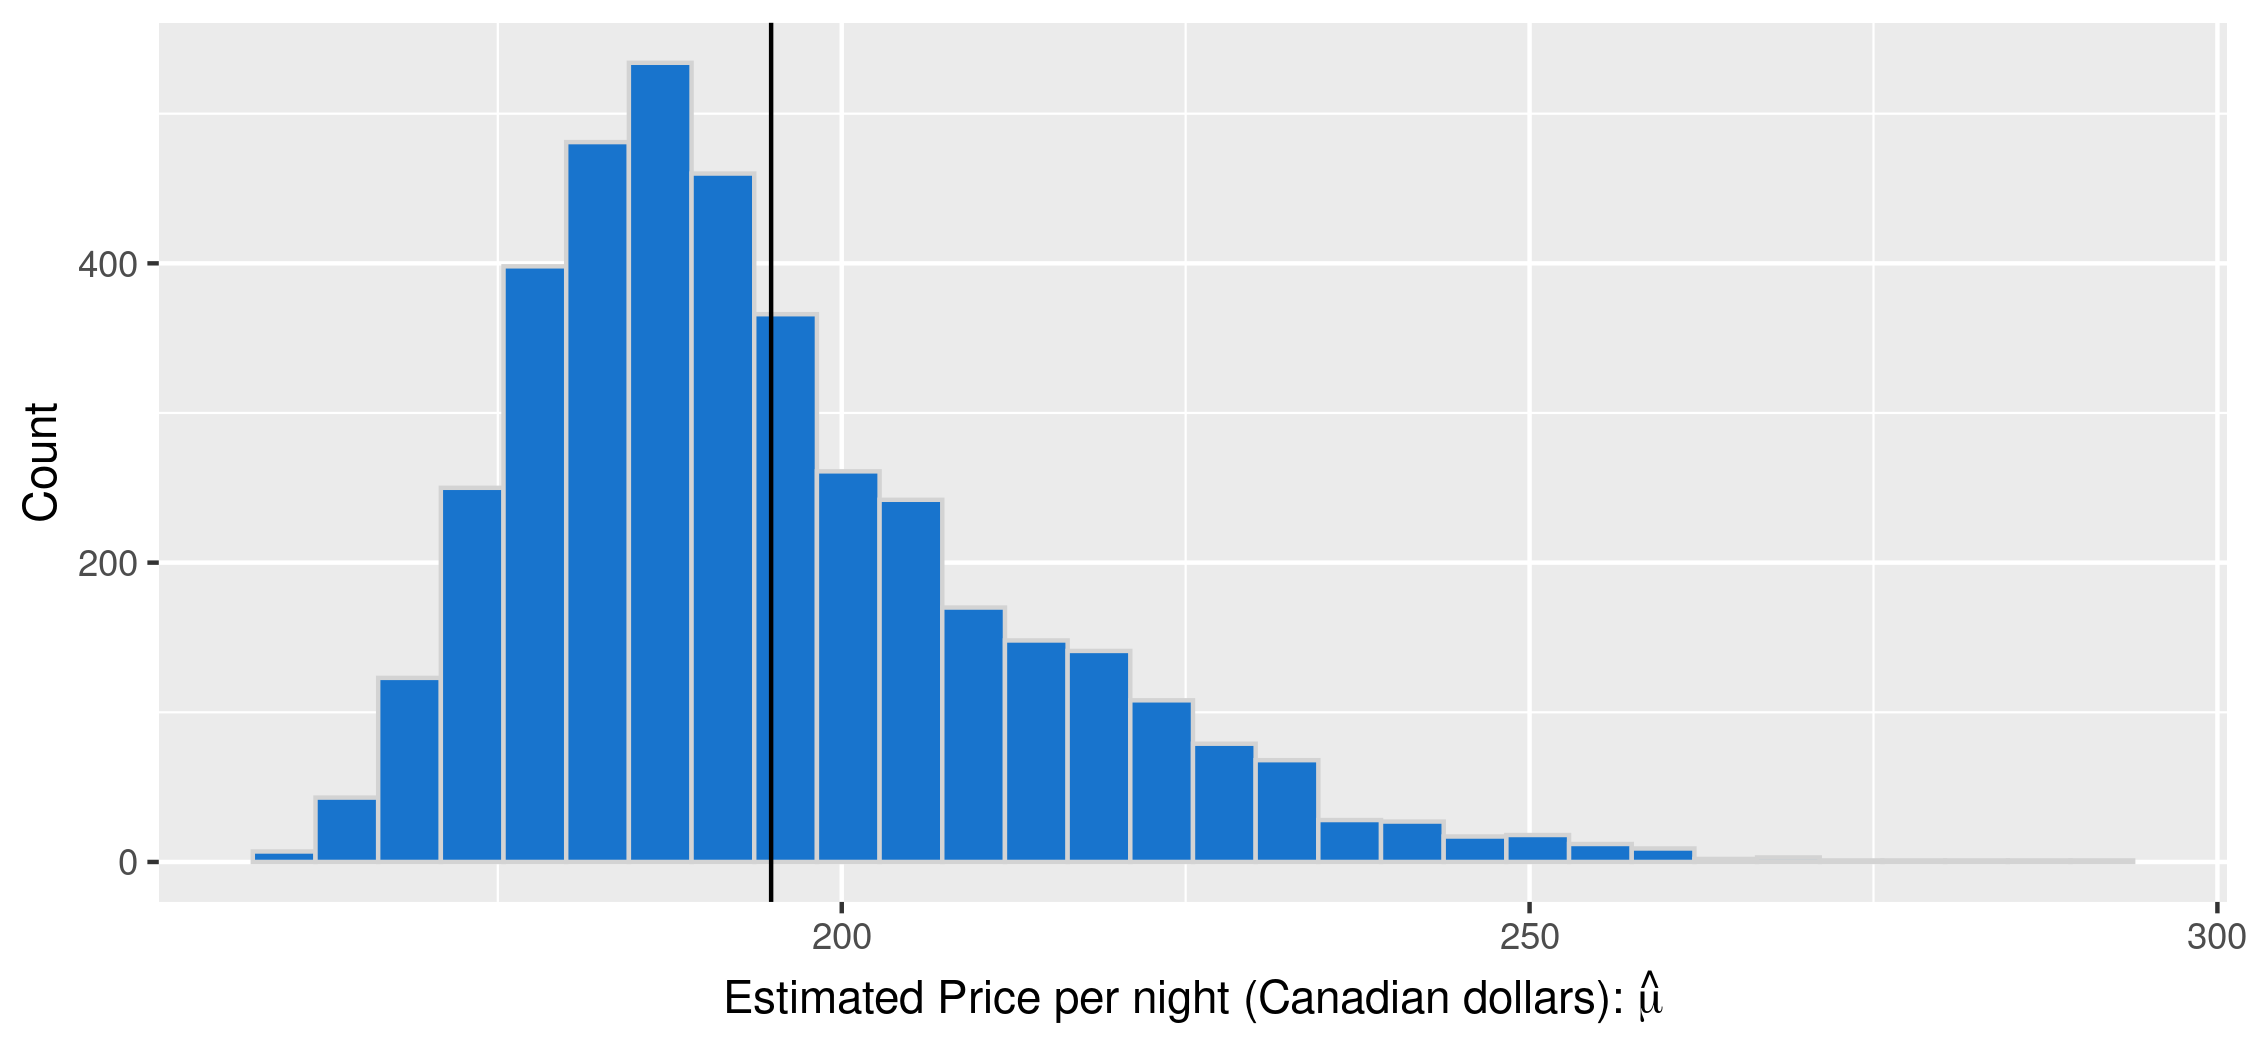
\includegraphics[width=0.98\linewidth,height=0.461\linewidth]{figure/base-hist-1} 

}



\end{knitrout}
}


\newcommand{\BaseHistogramWithArrow}{
\begin{knitrout}
\definecolor{shadecolor}{rgb}{0.969, 0.969, 0.969}\color{fgcolor}

{\centering 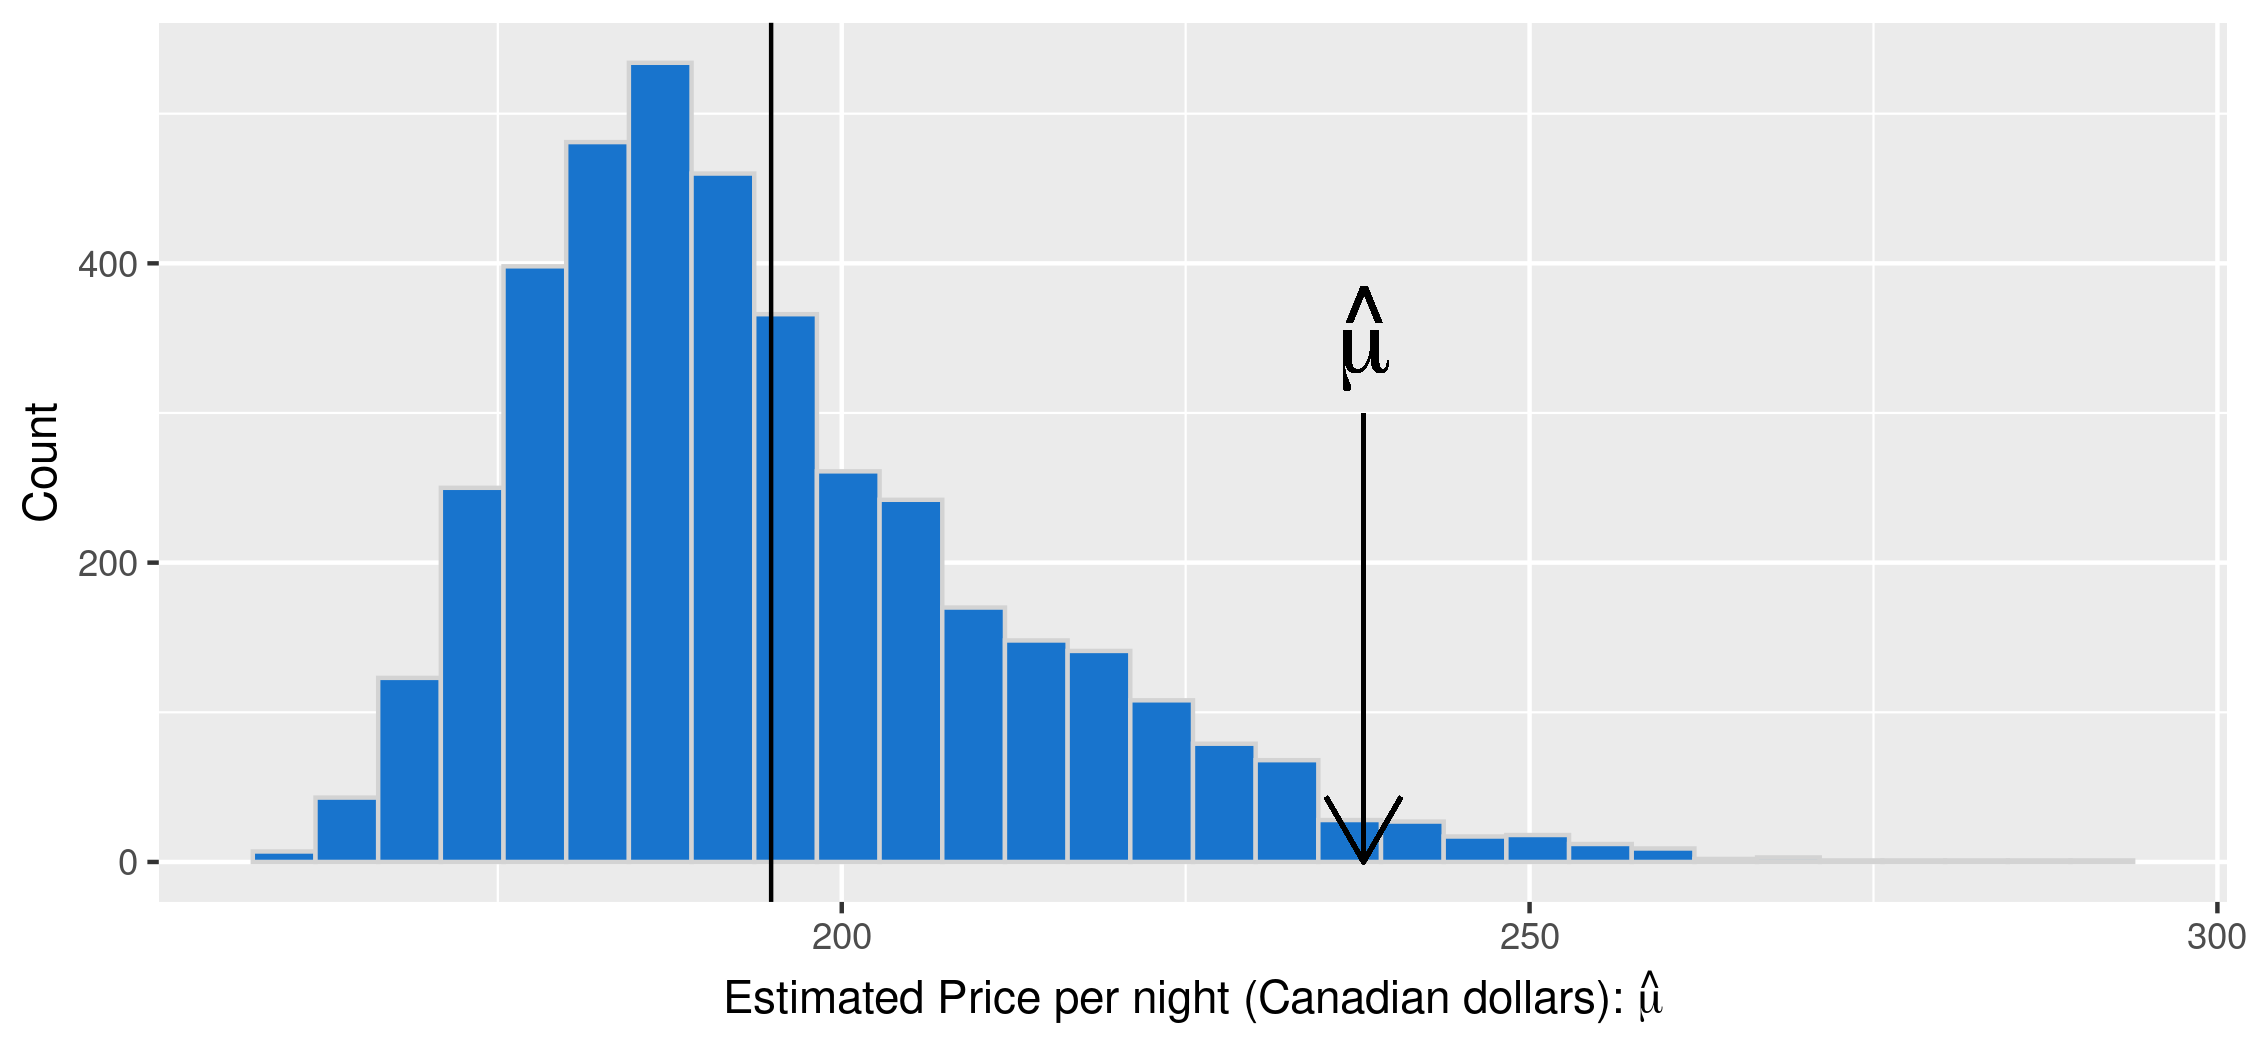
\includegraphics[width=0.98\linewidth,height=0.461\linewidth]{figure/base-hist-arrow-1} 

}



\end{knitrout}
}



\newcommand{\BaseHistogramFaded}{
\begin{knitrout}
\definecolor{shadecolor}{rgb}{0.969, 0.969, 0.969}\color{fgcolor}

{\centering 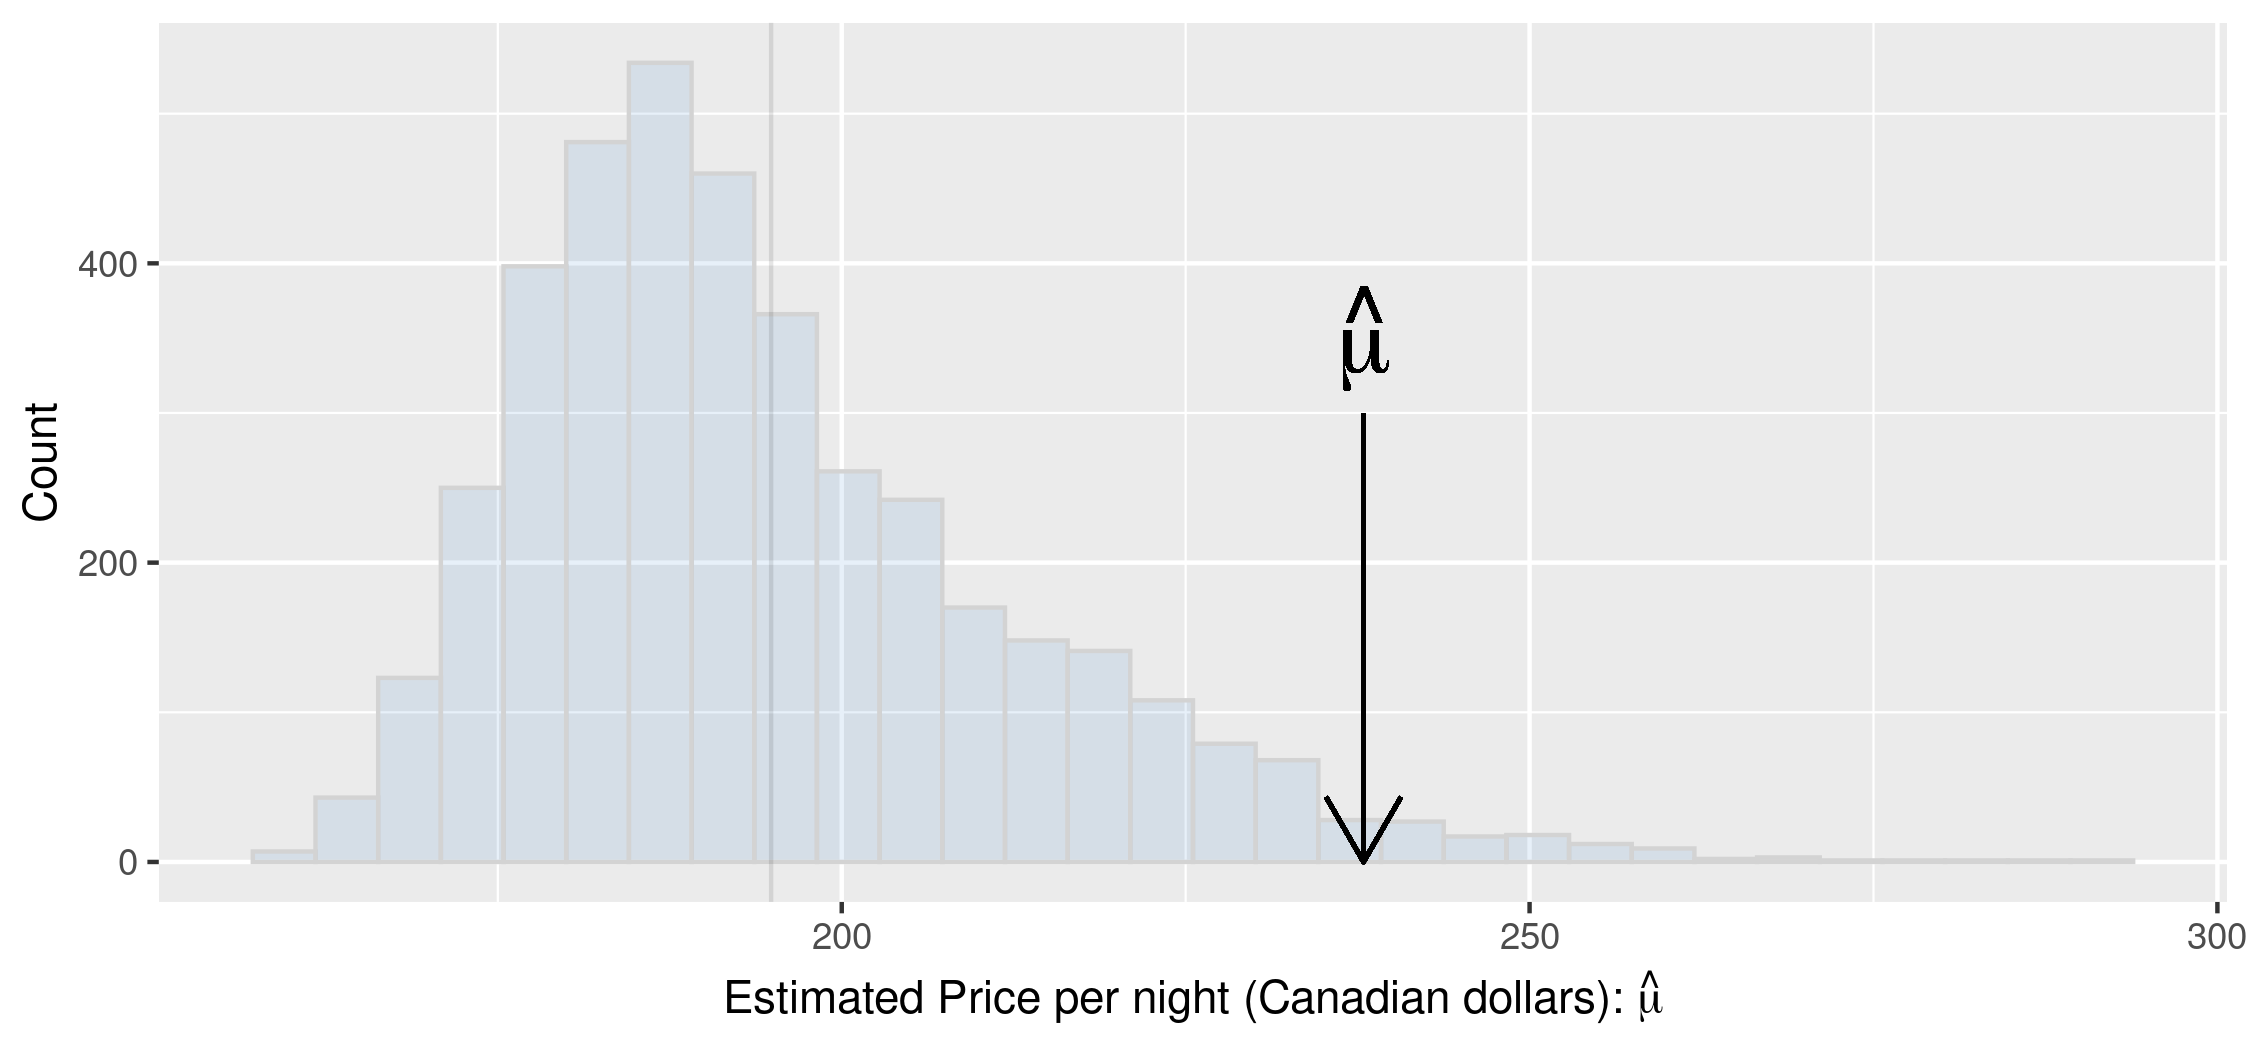
\includegraphics[width=0.98\linewidth,height=0.461\linewidth]{figure/base-hist-faded-1} 

}



\end{knitrout}
}


\newcommand{\SingleCI}{
\begin{knitrout}
\definecolor{shadecolor}{rgb}{0.969, 0.969, 0.969}\color{fgcolor}

{\centering 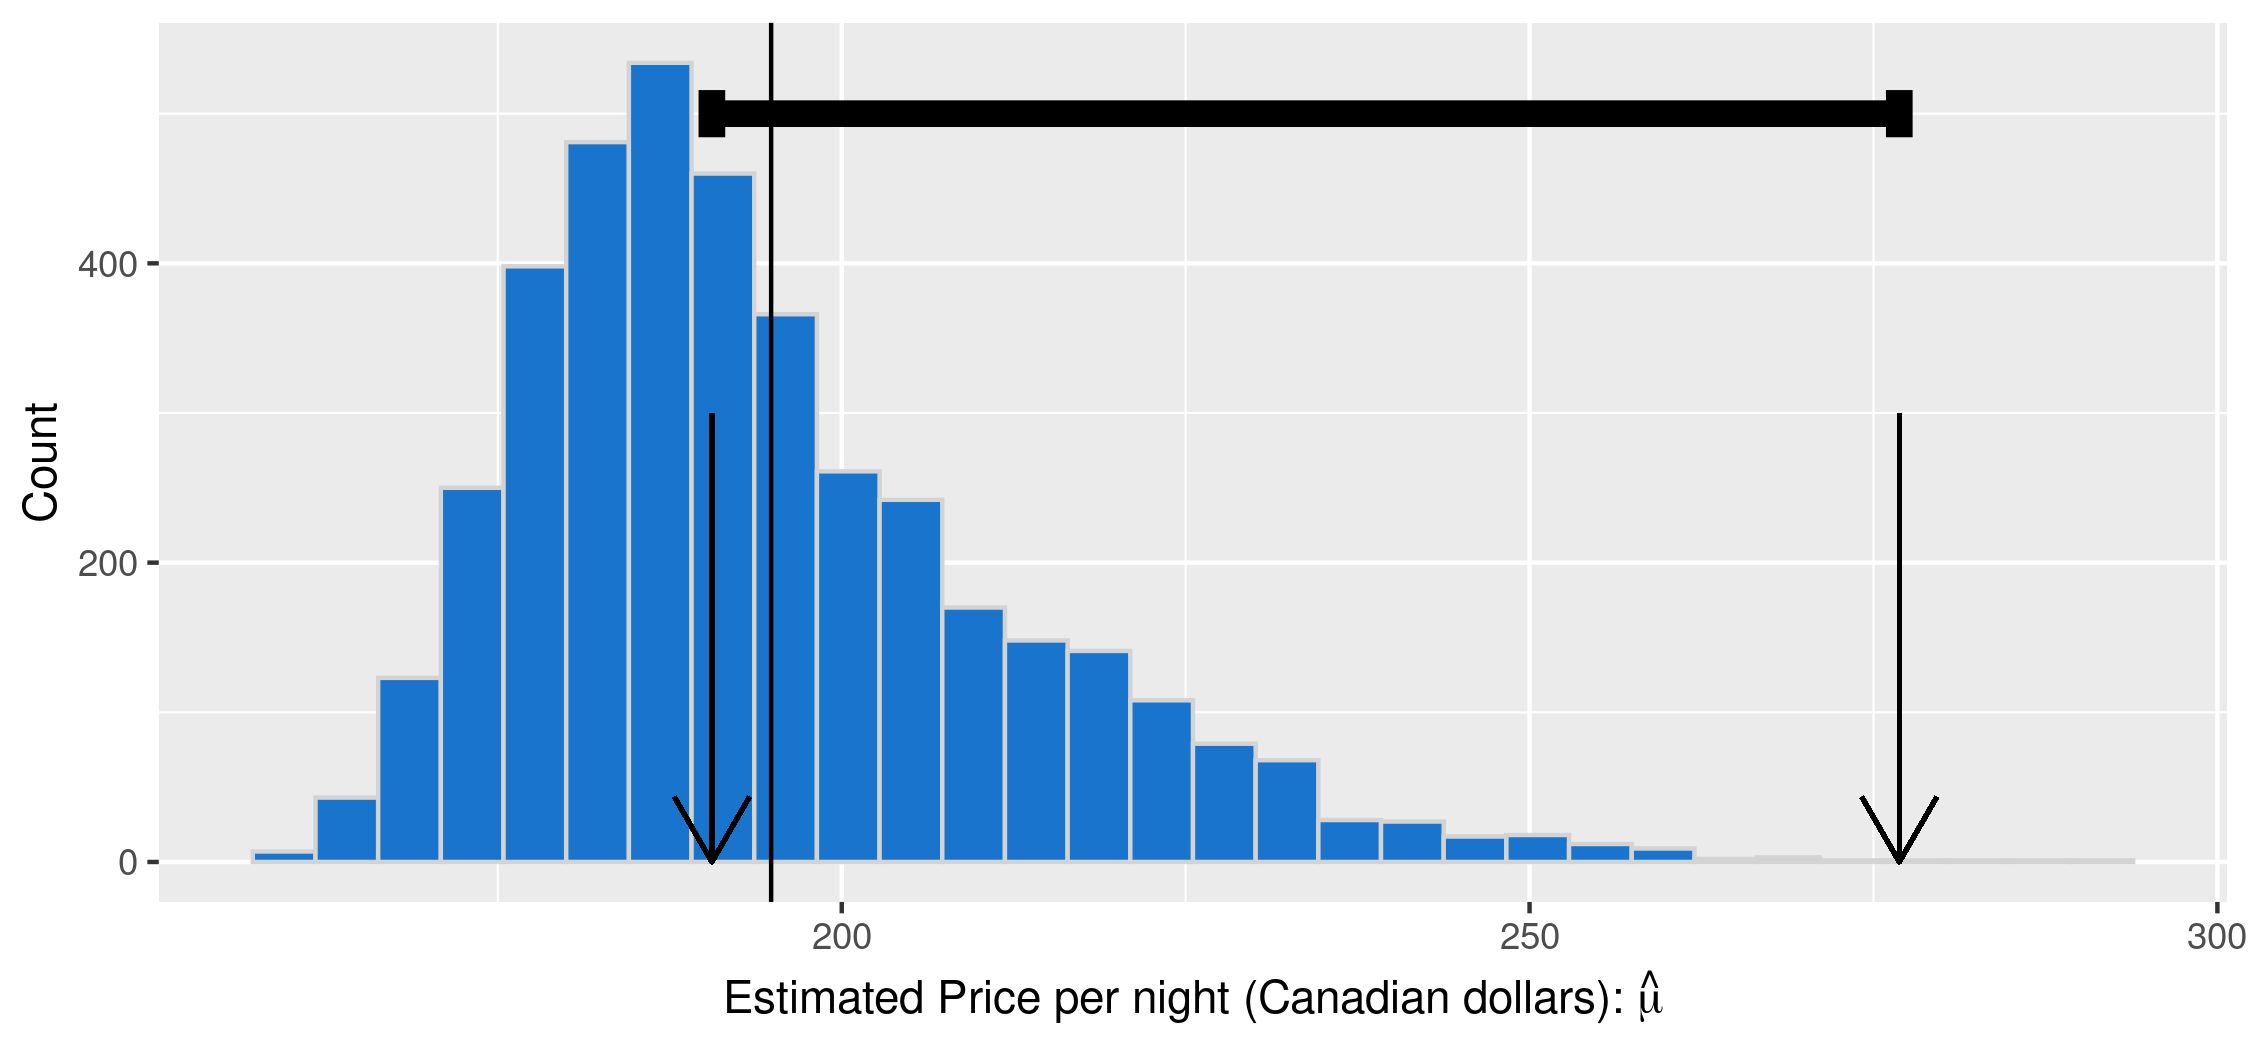
\includegraphics[width=0.98\linewidth,height=0.461\linewidth]{figure/base-hist-ci-1} 

}



\end{knitrout}
}




\newcommand{\SingleCIB}{
\begin{knitrout}
\definecolor{shadecolor}{rgb}{0.969, 0.969, 0.969}\color{fgcolor}

{\centering 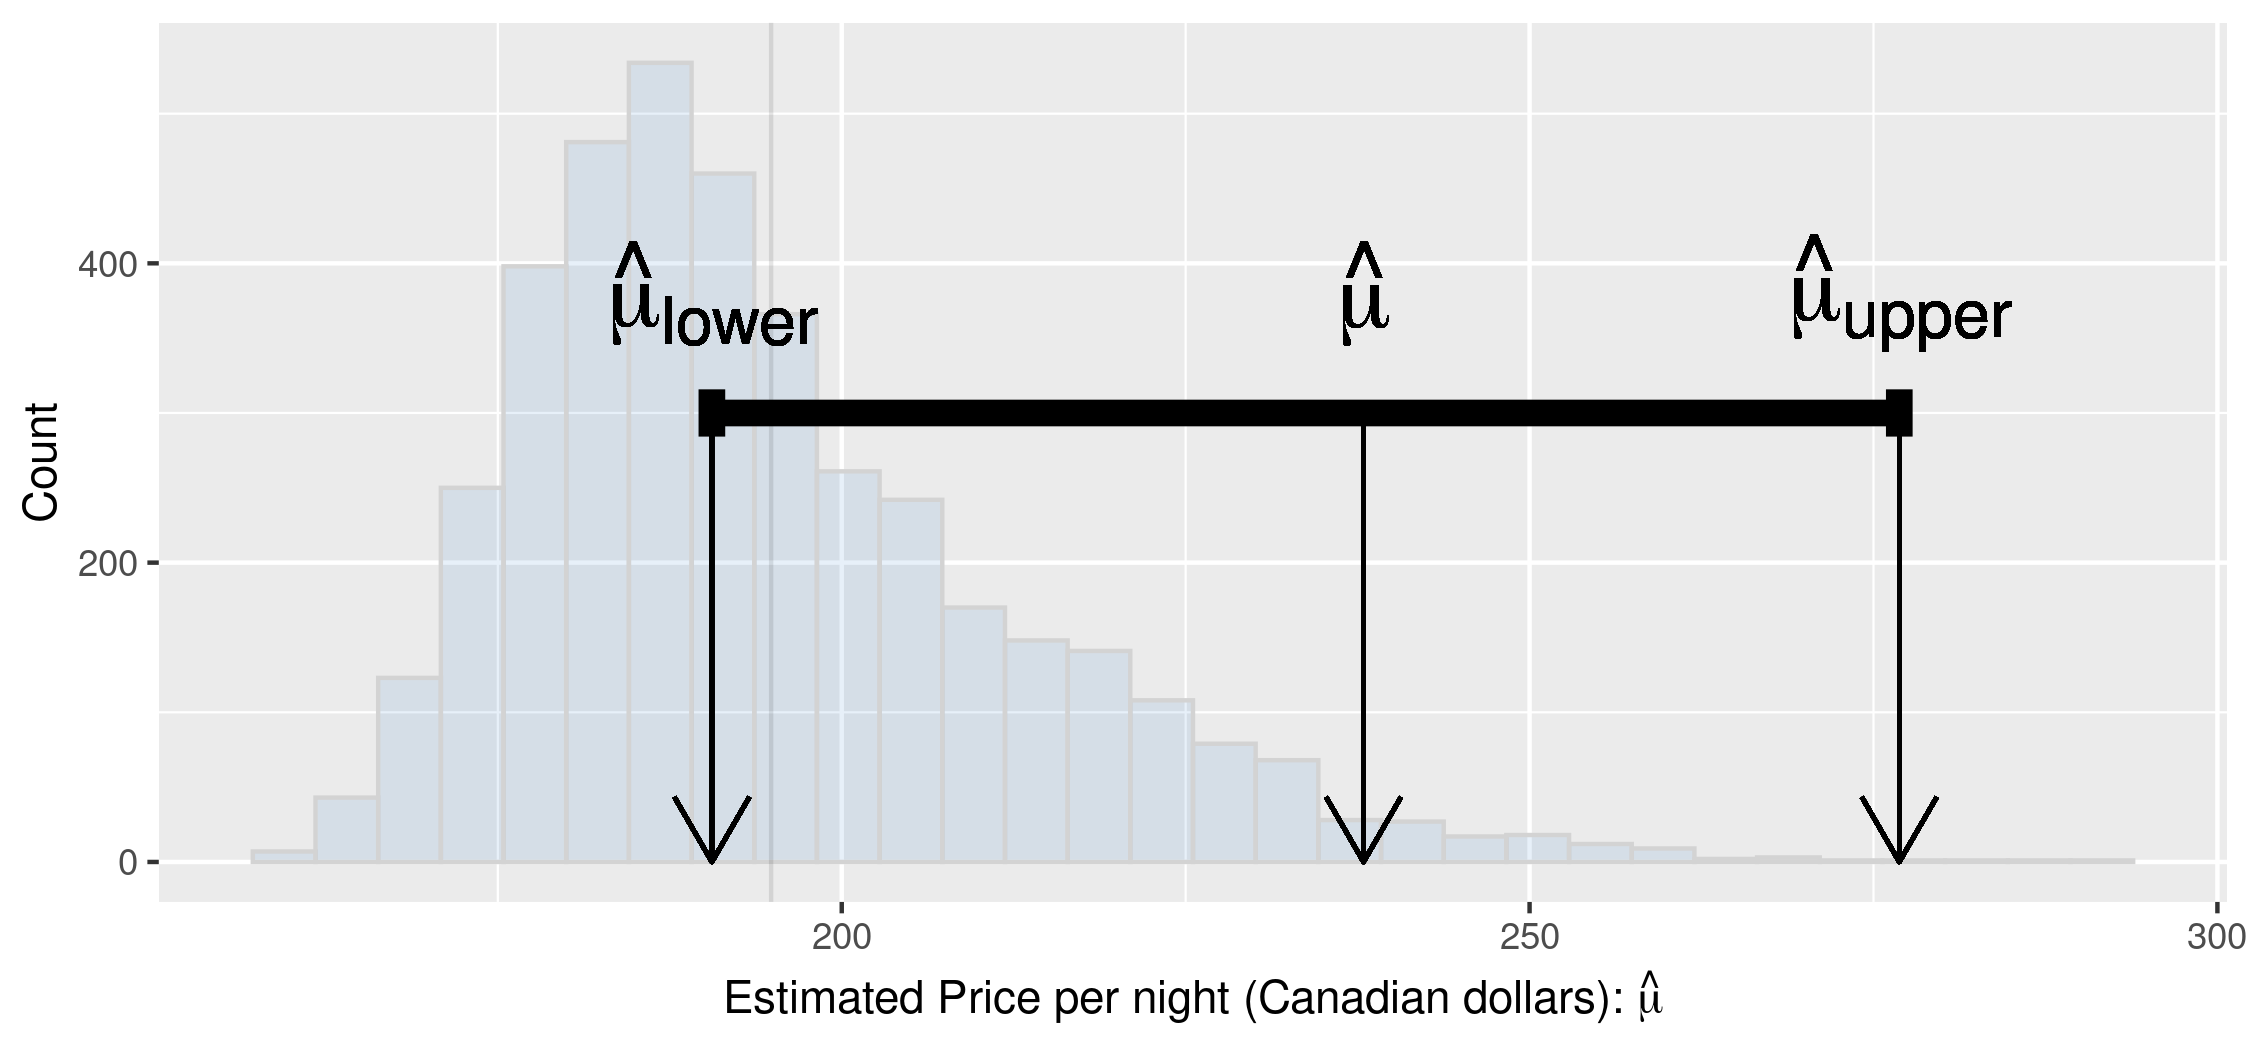
\includegraphics[width=0.98\linewidth,height=0.461\linewidth]{figure/base-hist-cib-1} 

}



\end{knitrout}
}



\newcommand{\MultipleCIs}{



\begin{knitrout}
\definecolor{shadecolor}{rgb}{0.969, 0.969, 0.969}\color{fgcolor}

{\centering 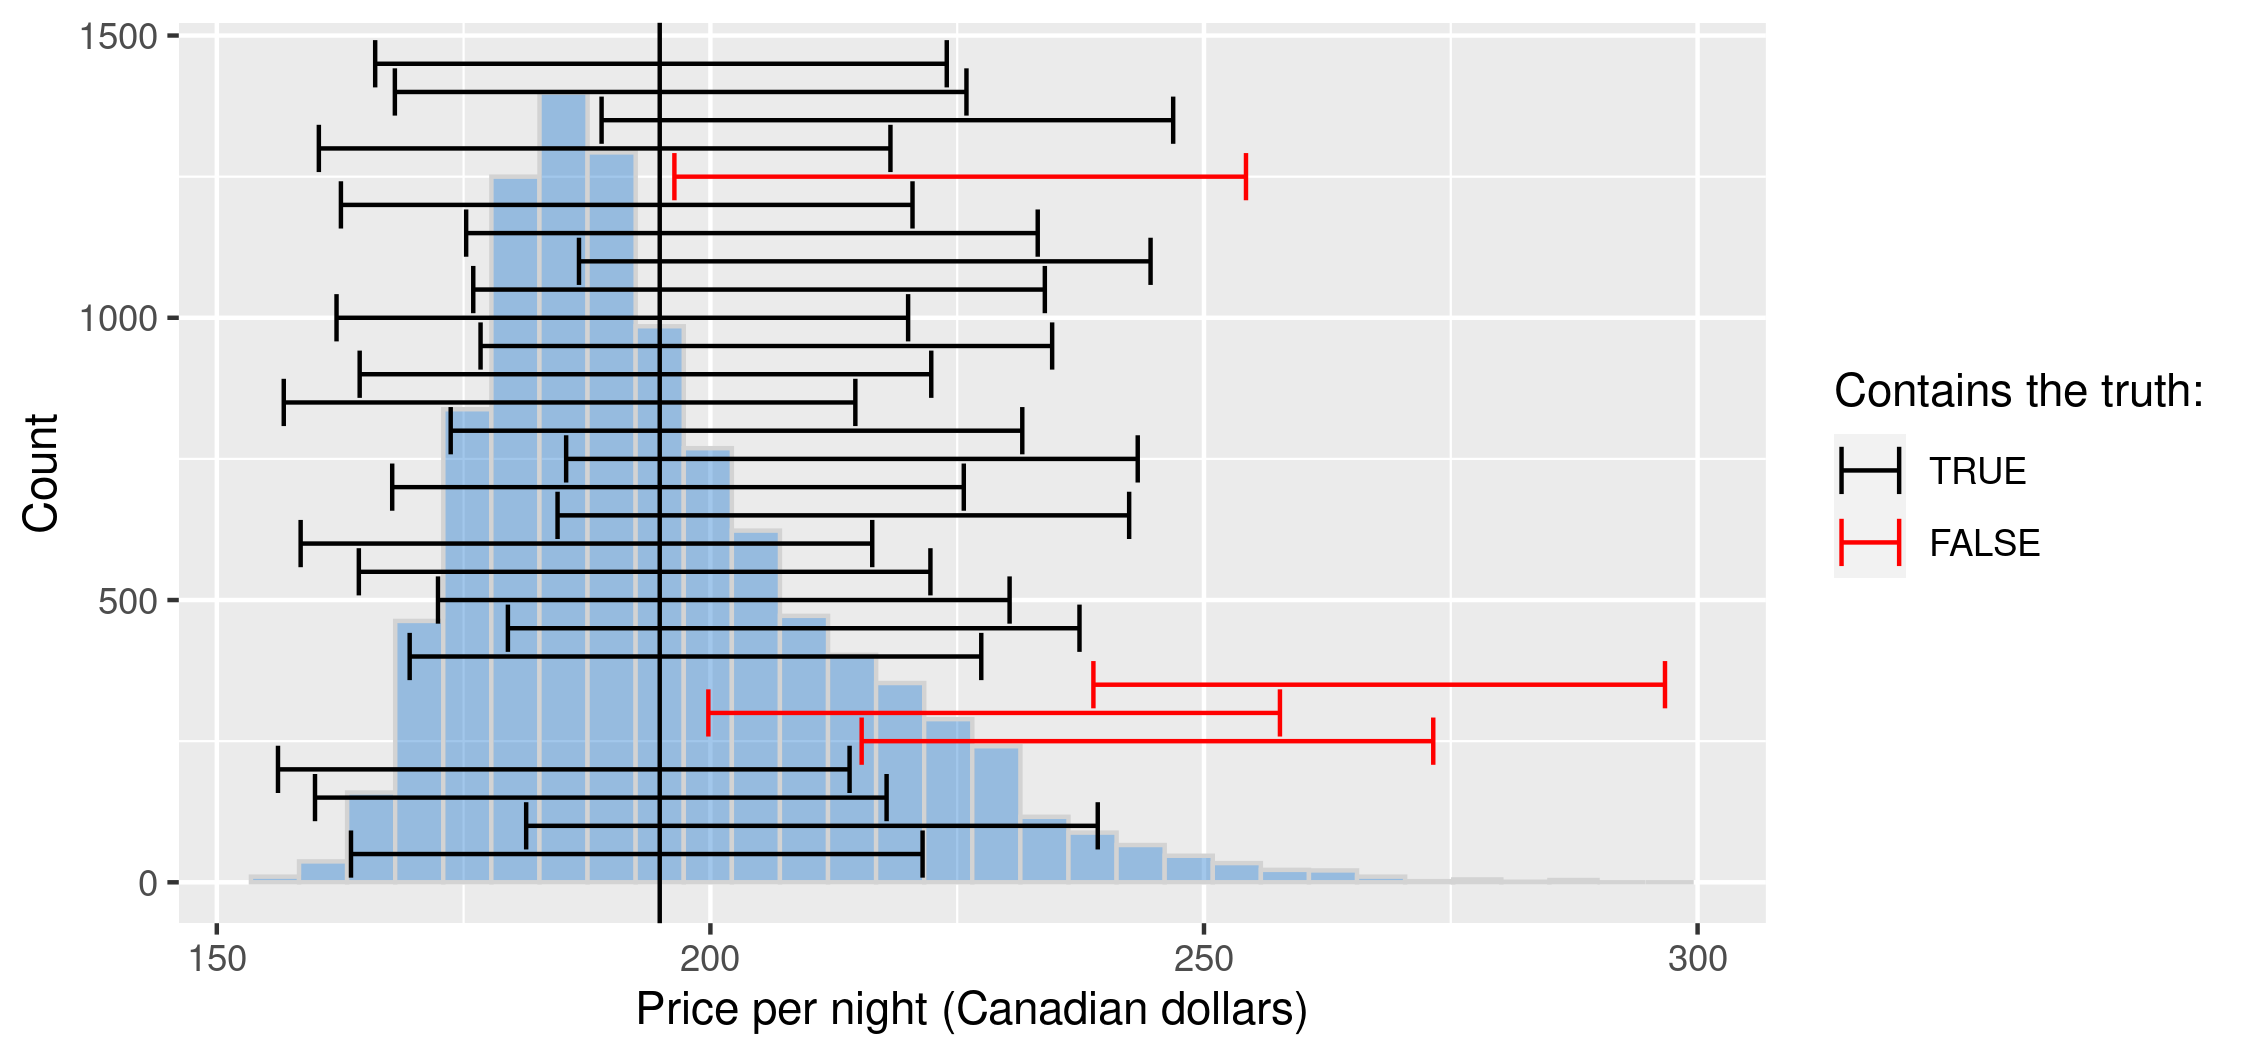
\includegraphics[width=0.98\linewidth,height=0.461\linewidth]{figure/base-hist-cis-1} 

}



\end{knitrout}
}


%%%%%%%%%%%%%%%%%%%%
% amsthm commands

\theoremstyle{plain}
\newtheorem{lem}{Lemma}
\newtheorem{thm}{Theorem}
\newtheorem{prop}{Proposition}
\newtheorem{cond}{Condition}
\newtheorem{assu}{Assumption}
\newtheorem{cor}{Corollary}
\newtheorem{conj}{Conjecture}

\theoremstyle{definition}
\newtheorem{defn}{Definition}
%\newtheorem{ex}{Example}

% Example environment with a terminating symbol.
% https://tex.stackexchange.com/questions/16453/denoting-the-end-of-example-remark
\theoremstyle{definition}
\newtheorem{examplex}{Example}
\newenvironment{ex}
  {\pushQED{\qed}\renewcommand{\qedsymbol}{$\triangle$}\examplex}
  {\popQED\endexamplex}


%%%%%%%%%%%%%%%%%%%%
% refstyle commands

\newref{event}{
    name=Event~, %
    names=Events~, %
    Name=Event~,
    Names=Events~
    }

\newref{item}{
    name=Item~, %
    names=Items~, %
    Name=Item~,
    Names=Items~
    }

\newref{fig}{
    name=Figure~, %
    Name=Figure~
    }

\newref{tab}{
    name=Table~, %
    Name=Table~
    }

\newref{sec}{
    name=Section~, %
    Name=Section~,
    names=Sections~, %
    Names=Sections~
    }

\newref{app}{
    name=Appendix~, %
    Name=Appendix~
    }

\newref{eq}{
    name=Eq.~, %
    Name=Eq.~,
    names=Eqs.~, %
    Names=Eqs.~
    }

\newref{fig}{
    name=Figure~, %
    Name=Figure~
    }

\newref{def}{
    name=Definition~, %
    Name=Definition~
    }

\newref{assu}{
    name=Assumption~, %
    Name=Assumption~,
    names=Assumptions~, %
    Names=Assumptions~,
    }

\newref{cond}{
    name=Condition~, %
    Name=Condition~,
    names=Conditions~, %
    Names=Conditions~
    }

\newref{prop}{
    name=Proposition~, %
    Name=Proposition~,
    names=Propositions~, %
    Names=Propositions~
    }

\newref{lem}{
    name=Lemma~, %
    Name=Lemma~,
    names=Lemmas~, %
    Names=Lemmas~
    }

\newref{ex}{
    name=Example~, %
    Name=Example~}

\newref{cor}{
    name=Corollary~, %
    Name=Corollary~
    }

\newref{thm}{
    name=Theorem~, %
    Name=Theorem~,
    names=Theorems~, %
    Names=Theorems~
    }

\newref{proof}{
    name=Proof~, %
    Name=Proof~
    }

\newref{conj}{
    name=Conjecture~, %
    Name=Conjecture~
    }

\newref{algr}{
    name=Algorithm~, %
    Name=Algorithm~,
    names=Algorithms~, %
    Names=Algorithms~,
    }


%% refstyle examples:
% \Secref[vref]{introduction} contains \secref{introduction}.
% \Secref[vref]{ack} does not contain \secref{introduction}.
%
% \begin{align}
%     x=y \eqlabel{myeq}
% \end{align}
%


\DefineMacros{}

\title{When Can Dropping a Little Data Make a Big Difference?}
\author{}
\date{May 5th, 2021}
% \institute{University of California, Berkeley}

\setbeamertemplate{Collaborators}[none]
\IfFileExists{upquote.sty}{\usepackage{upquote}}{}
\begin{document}

% \maketitle

\begin{frame}

\begin{center}
\large
\textbf{
An Automatic Finite-Sample Robustness Metric:
\\Can Dropping a Little Data Make a Big Difference?}
\end{center}

\hrulefill

Ryan Giordano (\texttt{rgiordan@mit.edu})\\
December 2021\\
% \vspace{5em}
% (Joint work with Rachael Meager and Tamara Broderick)
\end{frame}


\begin{frame}{Mister freakin P}


\end{frame}







%%%%%%%%%%%%%%%%%%%%%%%%%%%%%%%%%%%%%%%%%%%%%%%%%%%%%%%%%%%%%%%%%%%%%
%%%%%%%%%%%%%%%%%%%%%%%%%%%%%%%%%%%%%%%%%%%%%%%%%%%%%%%%%%%%%%%%%%%%%
%%%%%%%%%%%%%%%%%%%%%%%%%%%%%%%%%%%%%%%%%%%%%%%%%%%%%%%%%%%%%%%%%%%%%

\begin{frame}{Links and references}

\footnotesize

% {\bf A workshop paper: }\newline
Tamara Broderick, Ryan Giordano, Rachael Meager (alphabetical authors) \newline
``An Automatic Finite-Sample Robustness Metric: Can Dropping a Little Data Change Conclusions?''
\newline {\color{blue}\url{https://arxiv.org/abs/2011.14999}}

\par\noindent\rule{\textwidth}{0.4pt}

\bibliographystyle{plainnat}
% Hide the references header
% https://tex.stackexchange.com/questions/22645/hiding-the-title-of-the-bibliography/370784
\begingroup
\renewcommand{\section}[2]{}%
{
\tiny
%\scriptsize
\bibliography{bibliography}
}
\endgroup

\end{frame}

\end{document}
